% Drawing 69/02-4 -- folder 69, batch 02, archive page 28 (PDF page 29).
% Transcription: dans la marge gauche, sous « $D_4$ = « carrousel » » : un triangle $u, v, w$ ; de $w$ partent deux traits vers le bas, marqués $\lambda_w, \mu_w$ ; de $u$ deux traits vers $\lambda_u, \mu_u$, de $v$ deux traits vers $\lambda_v, \mu_v$
% Kind: triangle with pairs of pendant edges (carrousel). Method 2 (schematic redraw from the facsimile). Status: ok.
% Notes: Under "D_4 = carrousel": triangle u, v, w (w at the top); from each vertex two strokes go down, marked lambda, mu with the vertex index. The lower end labels are as the transcription reads them.
% Coordinates: 1 unit = 1 mm = 1/100 of the crop width (bbox in page fractions: [0.06, 0.2, 0.3, 0.34]).
% Redrawn by Claude (claude-opus-5-5), issue #73, 2026-11-07; not checked by a human; not compiled (no TeX in the session).
% Rights: reproduces part of the work -- behind RENDER_TRANSCRIPTS, never published by itself.
\documentclass[tikz,border=3pt]{standalone}
\usepackage{amsmath,amssymb}
\usetikzlibrary{patterns,arrows.meta}
\tikzset{pencil/.style={black!45}, struck/.style={black!35}, mark/.style={circle,draw,inner sep=1.3pt}, pt/.style={circle,fill,inner sep=0.9pt}, opt/.style={circle,draw,fill=white,inner sep=1.1pt}}
\begin{document}
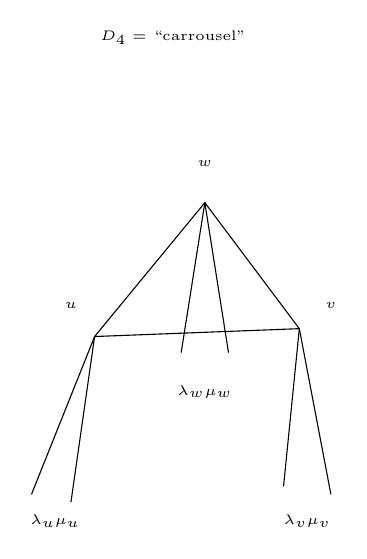
\begin{tikzpicture}[x=1mm,y=1mm,line cap=round,line join=round,font=\scriptsize]
\draw (52,-39) -- (38,-56) -- (64,-55) -- cycle;
\draw (52,-39) -- (49,-58);
\draw (52,-39) -- (55,-58);
\draw (38,-56) -- (30,-76);
\draw (38,-56) -- (35,-77);
\draw (64,-55) -- (62,-75);
\draw (64,-55) -- (68,-76);
\node[inner sep=1pt] at (52,-34) {\tiny $w$};
\node[inner sep=1pt] at (35,-52) {\tiny $u$};
\node[inner sep=1pt] at (68,-52) {\tiny $v$};
\node[inner sep=1pt] at (52,-63) {\tiny $\lambda_w\mu_w$};
\node[inner sep=1pt] at (33,-79.5) {\tiny $\lambda_u\mu_u$};
\node[inner sep=1pt] at (65,-79.5) {\tiny $\lambda_v\mu_v$};
\node[inner sep=1pt] at (48,-18) {\tiny $D_4 = $ ``carrousel''};
\end{tikzpicture}
\end{document}
